\documentclass[11pt,a4paper]{ivoa}
\input tthdefs

\usepackage[utf8]{inputenc}

\title{IVOA Provenance Data Model}

\ivoagroup{DM}

\author{Kristin Riebe}
\author{Michèle Sanguillon}
\author{Florian Rothmaier}
\author{Mathieu Servillat}
\author{Mireille Louys}
\author{Francois Bonnarel}

% \previousversion[????URL????]{????Funny Label????}
\previousversion[http://volute.g-vo.org/svn/trunk/projects/dm/provenance/description/ProvDM-0.1-20141008.pdf]{ProvDM-0.1-20141008.pdf}
       

% own definitions
\definecolor{todocolor}{rgb}{1,1,0.8}
\definecolor{darkred}{rgb}{0.6,0,0}
\definecolor{rose}{rgb}{1.0,0.88,0.88}
\definecolor{darkgrey}{rgb}{0.35,0.35,0.35}
%\newcommand{\TODO}[1]{%
%    \noindent%
%    \textcolor{todocolor}{\sffamily [\textbf{TODO:} #1]}%
%}

\newcommand{\TODO}[1]{%
    \noindent%
    \colorbox{todocolor}{%
            \parbox{0.85\linewidth}{\sffamily \textbf{TODO:}\\
            #1}
    }%    
    \vspace{2pt}

}

\newcommand{\Note}[1]{%
    \noindent%
    \textcolor{darkgrey}{{\sffamily Note:} \emph{#1}}%    
}


\newcommand{\paragraphlb}[1]{\paragraph{#1}\mbox{}\\} % paragraph with line break

\setlength{\fboxsep}{5pt}
%\setlength{\fboxrule}{1.5pt}
\newcommand{\warning}[1]{%
    \vspace{\baselineskip}
    \noindent
    \parbox{\linewidth}{%
        \colorbox{darkred}{%
            \parbox{0.7\linewidth}{\large \sffamily \textcolor{white}{Warning}}%
        }\\[-1pt]
        \noindent%
        \fcolorbox{darkred}{rose}{%
            \parbox{0.7\linewidth-2\fboxrule}{#1}%
        }%
    }%
    \vspace{\baselineskip}
}%

\begin{document}
\begin{abstract}
This draft is still an internal working draft, any comments welcome! 
The urls above also won't work yet, because this draft is only circulated 
via the volute-repository for now.

\warning{
    Everything described here is at a very 
    preliminary state and may change at any time!
}

\end{abstract}


\section*{Acknowledgments}

This document has been developed in part with support from the German
Astrophysical Virtual Observatory (BMBF Bewilligungsnummer 05A08VHA).

Thanks for fruitful discussions to (in alphabetical order):
Francois Bonnarel, Markus Demleitner, Jochen Klar, Gerard Lemson, 
Mireille Louys and Adrian Partl.



\section*{Conformance-related definitions}

The words ``MUST'', ``SHALL'', ``SHOULD'', ``MAY'', ``RECOMMENDED'', and
``OPTIONAL'' (in upper or lower case) used in this document are to be
interpreted as described in IETF standard, \citet{std:RFC2119}.

The \emph{Virtual Observatory (VO)} is
a general term for a collection of federated resources that can be used
to conduct astronomical research, education, and outreach.
The \href{http://www.ivoa.net}{International
Virtual Observatory Alliance (IVOA)} is a global
collaboration of separately funded projects to develop standards and
infrastructure that enable VO applications.


\section{Introduction}

In this document, we discuss a draft for an IVOA standard data model for describing the
provenance of data. We focus here on observational data, since provenance for
simulated data is already covered by SimDM 
\cite{std:SimDM}. However, the currently discussed version is abstract enough so that 
it could be applied to any kind of processes, including extraction of data from 
databases or even the flow of scientific proposals from application to 
acceptance and scheduling of the proposed observations.




\subsection{Role within the VO Architecture}
\TODO{Will be inserted later.}
% Skipping this for now. Let's not let this draft look more official than it 
% currently is.

%\begin{figure}
%\centering
%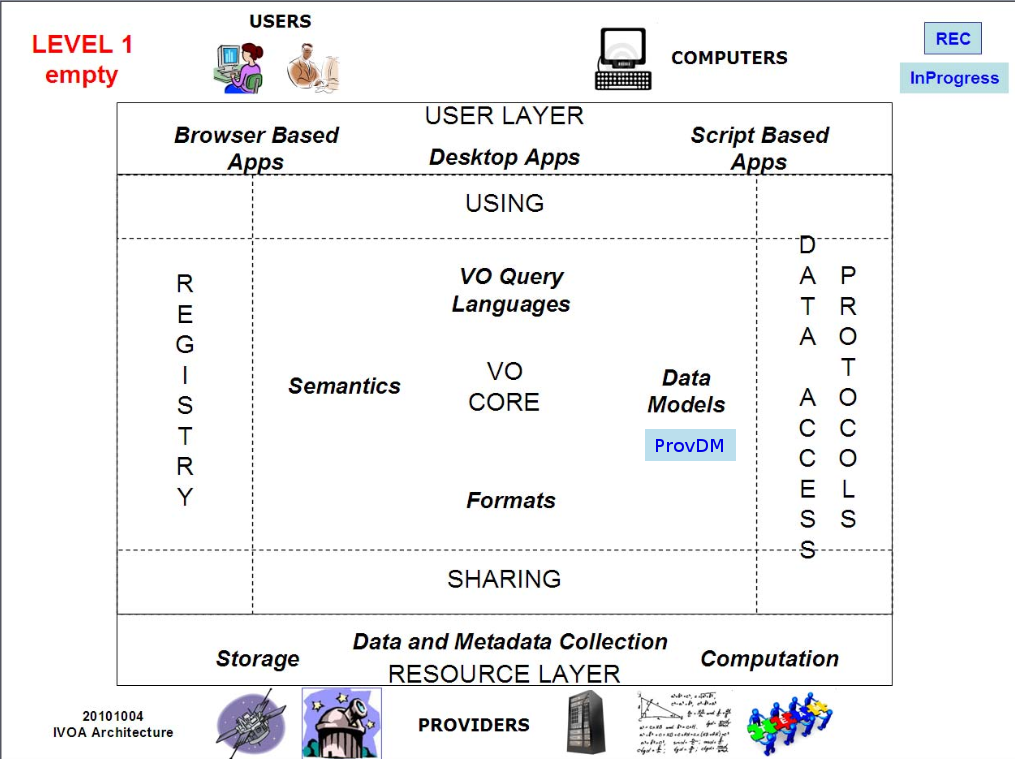
\includegraphics[width=0.9\textwidth]{archdiag.png}
%\caption{Architecture diagram for this document}
%\label{fig:archdiag}
%\end{figure}

%Fig.~\ref{fig:archdiag} shows the role this document plays within the
%IVOA architecture \citep{note:VOARCH}.


\subsection{Requirements for Provenance and Use Cases}
\subsubsection{Requirements}\label{sec:requirements}

An IVOA provenance data model should provide solutions to the following tasks:

\paragraphlb{A: Tracking the production history}
        Find out which steps were taken to produce a dataset and list the methods/tools/software that was involved. 
        Track the history back to the raw data files/raw images, show the workflow.

        \noindent Examples: 
        \begin{itemize}
            \item Is the image from catalogue xxx already calibrated?
What about dark field subtraction? Were foreground stars removed? Which technique
was used?  
            
            \item Is the background noise of atmospheric muons still present in my neutrino data sample?  
        \end{itemize}

        We don't go so far as to consider easy reproducibility as a use case -- this would be too ambitious. But at least the 
        major steps undertaken to create a piece of data should be recoverable.

      
\paragraphlb{B: Attribution and further information}
        Find the people involved in the production, the people/organizations/institutes that need to be cited or can be asked for more information.

        \noindent Examples: 
        \begin{itemize}
            \item I want to use an image for my own work -- who was involved in
creating it? Whom do I need to cite or who can I contact to get this information?  
            \item I have a question about column xxx in the data
table. Who can I ask about that?  
        \end{itemize}
      

\paragraphlb{C: Aid in debugging}
        Find possible error sources.

        \noindent Examples:
        \begin{itemize}
            \item I found something strange in an image. Where does
the image come from? Which instrument was used, with which characteristics
etc.? Was there anything strange noted when the image was taken?  
            \item Which pipeline version was used -- the old one
with a known bug for treating bright objects or a newer version?  
            \item This light curve doesn't look quite right. How was
the photometry determined for each data point?  
        \end{itemize}


\paragraphlb{D: Quality assessment}
        Judge the quality of an observation, production step or data set.
        
        \noindent Examples:
        \begin{itemize}
            \item Since wrong calibration images may increase the
number of artifacts on an image rather than removing them, the knowledge about
the calibration image set will help to assess the quality of the calibrated
image.  
        \end{itemize}
      

\paragraphlb{E: Search in structured provenance metadata}
        Find all images produced by a certain processing step and similar tasks.
        
        \noindent Examples:
        \begin{itemize}
            \item Give me more images that were produced using the
same pipeline.  
            \item Give me an overview on all images reduced with the same calibration data set.  
            \item Are there any more images attributed to this observer?  
            \item Which images of the crab nebula are of good quality and were produced within the last 10 years by someone not from ESO or NASA?  
        \end{itemize}

        This task is probably the most challenging. It also includes tracking the history of data items as in A, but we still have listed this task separately, since we may decide that we can't keep this one, but we definitely want A.

\subsubsection{User views on provenance}\label{sec:userviews}

The listed requirements/use cases were collected having an external scientist in mind who retrieves data from the virtual observatory and needs to get more background information. When looking at internal processes, one can also use provenance for checking workflows, e.g. if reduced images from a pipeline don't look quite right, the pipeline can be re-run with different parameters. Tracking the workflow in a common provenance description can help to quickly identify the problematic parameters and to keep a better track of changes. It can also be used to exchange pipeline recipes between different projects in a standardized way.

Thus, we could classifiy different views on the provenance information:
\begin{itemize}
\item \textbf{basic view}: This gives just the main datasets and activities or only collections of them, if they exist, and their relations. This provides an overview on the main steps and could be converted into a figure for e.g. project reports with existing PROV-tools (e.g. ProvStore(\url{https://provenance.ecs.soton.ac.uk/store/} or the prov-Python package \url{https://pypi.python.org/pypi/prov})  

\item \textbf{detail view}: This gives e.g. an external scientist enough information to track back the history of one given entity, e.g. an observation-entry in a table, a file or an image. Most external scientists are probably only interested in science-ready data, so maybe there is no need to show all details for e.g. uncalibrated raw images.

\item \textbf{full view}: A full view would be required for scientists who want to use the information to reprocess data from the beginning, i.e. they may need all the information including e.g. raw images from observations and which flat-fields were taken etc.
\end{itemize}

\Note{Maybe split this section into 1) use case: different users have different needs, which appears here and 2) define different views on provenance, which should be put into a different section in the main part, not in introduction.}


\subsubsection{More specific use cases}
More specific use cases with example serialisations for different types of astronomical data sets are given in Section \ref{sec:examples}.
    

\subsubsection{Further possible applications}

The provenance of the flow of scientific proposals at observatories could also be tracked using the core provenance model. The provenance information could be used to check internal processes, e.g. if the proposal was approved by a person from a certain committee, if the time span between application and acceptance/refusal does not extend a certain period etc. 


\subsection{Goal of the provenance model}
The goal of the provenance data model is to describe how provenance information can be modeled and stored/exchanged within the virtual observatory. Its scope is mainly to allow modelling of the flow of data, the relations between data and processing steps. Characteristics of observations like ambient conditions and instrument characteristics won't be modeled here explicitely. They are to be included in the form of data sets (entities) only.


\subsection{Previous efforts}

Outside of the astronomical community, the Provenance Challenge series (2006 - 2010), a community effort to achieve inter-operability between different representations of provenance in scientific workflows, resulted in the Open Provenance Model (\cite{moreau2010}). 
Later, the W3C Provenance Working Group was founded and released the W3C Provenance Data Model as Recommendation in 2013 (\cite{std:W3CProvDM}). 
OPM was designed to be applicable to anything, scientific data as well as cars or immaterial things like decisions. With the W3C model, this becomes more focused on the web.  Nevertheless, the core concepts are still in principle the same in both models and very general, so they can be applied to astronomical data sets and workflows as well. 
The W3C model was taken up by a larger number of applications and tools than OPM, we are therefore basing our modeling efforts on the W3C Provenance data model, making it less abstract, more specific or extend it where necessary. 


The W3C model even specifies already PROV-DM Extensibility points (section 6 in \cite{std:W3CProvDM}) for extending the core model. This allows to specify additional roles and types to each entity, agent or relation using the attributes \texttt{prov:type} and \texttt{prov:role}.
By specifying the allowed values for the IVOA model, we could adjust the model to our needs while still being compliant to W3C.


\section{A provenance data model}
\subsection{Overview - W3C core}\label{sec:w3c_overview}
We describe here the core concepts for modelling provenance. The resulting model can then be reused as a pattern everywhere where provenance
is needed in the VO. Some examples for different use cases are given in Section \ref{sec:examples}.

The elements of a provenance model can be expressed as a directed graph to capture the causal dependencies. 
Based on the W3C PROV-DM, we identified the need for the same three core elements, which represent the nodes of a provenance graph
(see Section 1+2 and Fig. 1 in \cite{std:W3CProvDM}). We list them here briefly with examples from the Astronomy domain, and will discuss them in detail later on.

\begin{itemize}
\item \emph{Entity:} a thing at a certain state\\
    examples: data products like images, catalogs, parameter files, calibration data, instrument characteristics

\item \emph{Activity:} an action/process or a series of actions, occurs over a period of time, performed on or caused by entities, usually results in new entities\\
    examples: data acquisition like observation, simulation; regridding, fusion, calibration steps, reconstruction

\item \emph{Agent:} executes/controls an activity, is responsible for an activity or an entity\\
    examples: telescope astronomer, pipeline operator, principal investigator, software engineer

\end{itemize}

\noindent
There are also different possible relations between these components. The main important core relations are:
\begin{itemize}
\item \emph{Generation:} a new entitiy is generated by an activity\\
        (output\_data wasGeneratedFrom activity)
\item \emph{Usage:} an entity is used by an activity\\
        (activity used input\_data)
\item \emph{Association:} agents have responsibility for an activity\\
        (agent wasAssociatedWith activity)
\item \emph{Attribution:} an entity can be attributed to an agent (entity wasAttributedTo agent)
\end{itemize}

Figure \ref{fig:w3cclasses} summarizes these (core) classes and relations of the W3C provenance model that are interesting for us.
Its components are discussed in more detail with respect to the role they play in provenance for the virtual observatory in the next section.

\begin{figure}
\centering
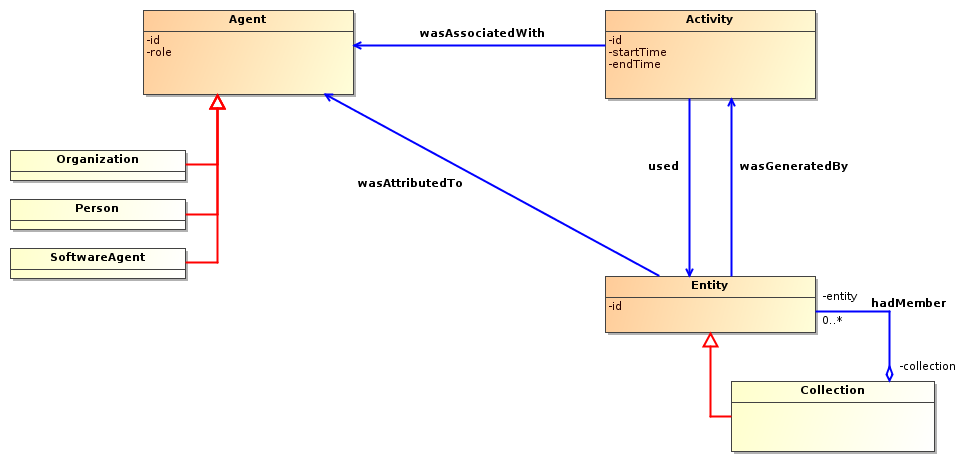
\includegraphics[width=0.8\textwidth]{ProvDM-W3C-classdiagram.png}
\caption{The main core classes and relations of the W3C Provenance Data Model.}
\label{fig:w3cclasses}
\end{figure}


\TODO{Decide, which elements of W3C-PROV are needed, what else to include here.}


\subsection{Detailed discussion of the W3C data model}
%We are now going to discuss each component and relation in more detail.

\subsubsection{Entity}
Entities in the VO are usually (astronomical/astrophysical) data sets in the form of images, tables, numbers, etc.. But they can also be observation/simulation log files, observation proposals, scientific articles or manuals and other documents. The Dataset Data Model \citep{std:DatasetDM} specifies an IVOA Dataset as ``a file or files which are considered to be a single deliverable''. An entity is not restricted to files. It can even be just a number in a table, depending on how fine-grained the provenance shall be described.

As a side-remark: according to the W3C model,  provenance information can also be an entity itself, with the \texttt{prov:type} ``Bundle''.

For each entity, we should store a number of attributes:
\begin{itemize}
\item id: a unique id for this entity (unique in its realm)
\item prov:label: a label (to be displayed by clients)
\item prov:type: a provenance type, i.e. one of: prov:collection, prov:bundle, prov:plan; 
\item dataProductType: could refer to something in the ObsCore data model \citep{std:ObsCore}; describes, what kind of product it is (e.g. image, table)
\item datatype: type of the physical representation of the entity, e.g. binary file, fits file, database, database table, ASCII file, tar-file, directory, integer, float
\item prov:description: text describing the entity in more detail
\item prov:location: (or storage or accessReference?) where the entity can be found
\end{itemize}

Possible further attributes could include  ``access'' (``public'' or ``restricted'' or 
``internal'') or how to access data on a certain machine etc.

The difference between entities that are used as input data or output data 
becomes clear by specifying the relations between the data and activities producing/using these data.

\subsubsection{Activity}
Activities in the VO include all steps in the reduction of images and production of new data sets, like image calibration, bias subtraction, image stacking; light curve generation from a number of observations, radial velocity determination from spectra, etc.

\begin{itemize}
\item For each data flow it should be possible to clearly identify entities and activities. If the activities shall not be recorded explicitely, one can also use the \emph{Derivation}-relation (see below) to link derived entities to their originals.

\item Data entities are results from activities (\emph{wasGeneratedBy}-relation), and can be used as input for other activities (\emph{used}-relation). 
%The difference between input data and output data becomes clear by specifying the relations. 

\end{itemize}

The W3C provenance model requires for activities an id, a startTime and endTime. 
Here's a list of useful further attributes for activities:

\begin{itemize}
\item id
\item prov:label
\item prov:type: one of the processes from a vocabulary or list, e.g. observation, reduction, calibration, publication
\item prov:description
\item prov:startTime
\item prov:endTime
\item docuLink: link to further documentation on this process, e.g. a paper, the source code in a version control system etc.
\end{itemize}

A ``version'' attribute could also be useful.



\subsubsection{Agent}\label{sec:w3c-agent}
An agent can be an organization or a person, and can take different roles for an activity or an entity. The possible types of agents are:
\begin{itemize}
\item prov:person: a person, specified by first and last name, email address, possibly also by affiliation (though all these parts may change in time)
\item prov:organization: a publishing house, institute, scientific project
\item prov:SoftwareAgent: still needs to be discussed
\end{itemize}

A definition of organizations in the sense of the VO is given in the IVOA Recommendation on Resource Metadata \citep{std:ResourceMeta}, hereafter refered to as RM. This also specifies that scientific projects can be considered as organizations on a finer lever.

There can be more than one agent for each activity/entity (with different roles) and one agent can be responsible for more than one activity/entity. This many-to-many relationship could be made more explicite by adding role-maps for agents explicitely in the UML-class diagram, as ``qualifiers'' for the relations. The W3C PROV-DM document specifies two relations instead, which we can extend with a ``role'' attribute as well. These are:

\begin{itemize}
\item wasAssociatedWith: relates an \emph{activity} to an agent
\item wasAttributedTo: relates an \emph{entity} to an agent
\end{itemize}

Note that the attributed-to-agent for a dataset may be different from the agent that is associated with the activity that created an entity. Someone who is performing a task is not necessarily given full attribution, especially if he acts on behalf of someone else.

In order to make it clearer what an agent is useful for, we suggest here possible roles an agent can have (along with descriptions partially taken from RM)\\
\begin{center}
\begin{tabular}{l|l|p{0.5\textwidth}}
\multicolumn{3}{c}{\textbf{AgentRoles}}\\ \hline
\textbf{prov:role} & \textbf{prov:type} & \textbf{Comment} \\ \hline
author & prov:person & someone who wrote an article, software, proposal\\
contributor & prov:person & someone who contributed to something (but not enough to gain authorship)\\
curator & prov:person & someone who checked and corrected a dataset before publishing\\
editor & prov:person & editor of e.g. an article, before publishing\\
publisher & prov:organization & organization (publishing house, institute) that published something\\
observer & prov:person & observer at the telescope\\
operator & prov:person & performing a given task (executor?)\\
coordinator/PI & prov:person & someone coordinating/leading a proje'ct\\
provider & prov:organization & ``an organization that makes data and/or services available to users over the network'' (definition from RM)
%& prov:project & the project for which certain tasks are done, which published the data, etc.\\
\end{tabular}
\label{tab:agentroles}
\end{center}
This list is not complete. Such roles are domain-specific and thus not fixed in W3C's PROV-DM. However, since we are considering here the Astronomy-domain, we could 
consider fixing these roles, most likely by keeping them in a vocabulary list.

\TODO{Do we have a specific use case for fixing the agent-roles? Is anyone going to search for specific roles in the Provenance meta-data?
Or shall we leave it open, which roles can be defined and just give examples here?}

\TODO{Do we need to fix the prov:types to the given roles? Or leave it free?}

\TODO{We still need to clarify precisely, in which way a \emph{software agent} is distinct from an activity.}


\subsubsection{Roles of entities}
\TODO{Probably these roles are best stored with the used/wasGeneratedBy relation directly.}
The W3C PROV-DM specifies a \textbf{Derivation} relation, which directly links a derived entity to its predecessor. This was introduced to make the link between entities more explicite. If activity a1 used entities e1 and e2 as input and produced e3 as output, then it is not clear, if e3 is a derivative (or, in W3C terms, ``wasDerivedFrom'') of e1 or if it was derived from e2 or from both or neither. e1 and e2 could have been only parameter files for an observation.  

However, for the IVOA provenance model we currently favour adding a \emph{role} to each data item or entity, which can explain in more detail in which way the entity was used.

We will discuss later an approach using the additional Method-class as prototype or template for each activity.
The types of input/output data and their roles are described using additional classes for the method, so that any kind of relation between input/output data can be covered.

One of the important details here is that e.g. many data sets used by one activity may have different roles for that process (one file is a parameter file, another one is the raw image, and the third one is the dark field that should be subtracted). Since these roles are very important for an activity, they have to be included in the provenance model.

These roles don't have to be unique (see \cite{moreau2010}, after Definition 10), many data sets may have the same role for a process (e.g. raw image input).

Each activity requires specific roles for each entity (provided in the used- or wasGeneratedFrom-relation). 

\TODO{In order to facilitate interoperability, for each activity, the possible entity-roles could be defined and described by the IVOA community, in a vocabulary list or thesaurus.}


\subsubsection{Mapping classes and input/output data}
We could adjust the W3C model by 
replacing the used- and wasGeneratedBy-relations by a mapping class between activity and entity in the class diagram in Figure~\ref{fig:classes-w3c-adjusted}, for making the possible \emph{roles} of input and output data more specific.

\begin{figure}
\centering
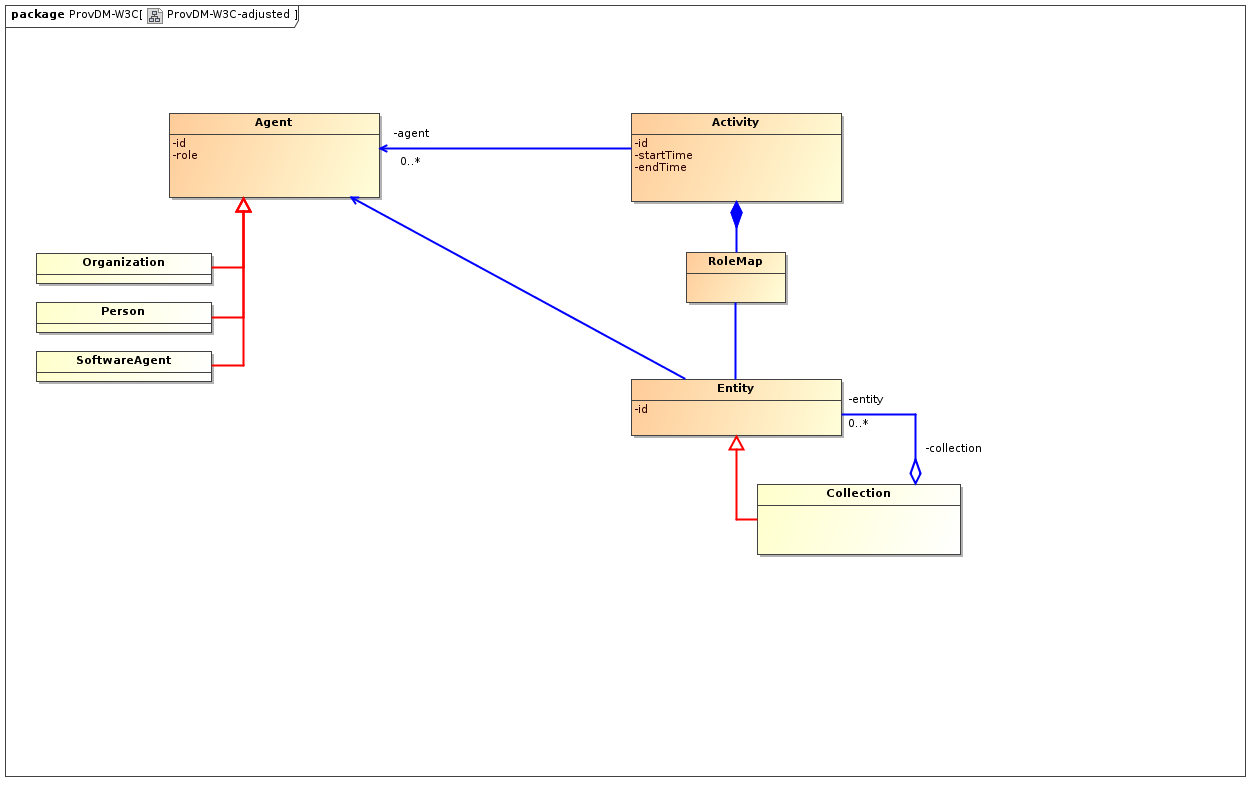
\includegraphics[width=0.8\textwidth]{ProvDM-W3C-adjusted.png}
\caption{An adjusted W3C model for provenance of astronomical data.}
\label{fig:classes-w3c-adjusted}
\end{figure}


The different methods and data types are here hidden in pre-defined vocabulary lists. 
An example for writing down the provenance for a stacked image in W3C and with the protoype-model (which is discussed in a later section) is given in the accompanying files 
\texttt{prov-example-incl-prototypes.txt} and 
\texttt{prov-example-w3c.txt} at \href{https://volute.g-vo.org/svn/trunk/projects/dm/provenance/description/}{volute}.


% The derivation relation together with entities is already enough to produce a data flow view, but in Astronomy we are probably even more interested in the Processes (as discussed in our first draft for requirements for provenance).


\subsubsection{Collection}
W3C describes a collection as an aggregation of entities. This is a useful concept to adapt here, since it allows to treat many data (e.g. a RAVE data set containing data tables and spectra) and then define provenance for this complete bundle. Therefore we included the ``Collection''-object into our class diagrams. A Collection is an entity, and has ``hadMember'' relations to each of its members.

The advantage is, that one can describe the provenance workflow on a coarser level, just using collections and the activities that created them. If users ask for more details on specific data sets one would additionally include the hadMember-relations to get the full provenance. Thus it allows us to hide complexity where necessary, i.e. to adjust the granularity of the provenance (also see Section \ref{sec:userviews}).

On the other hand, defining for each member of a collection a hadMember-relation can 
become quite cumbersome and will not look much more concise than writing the used- or wasGeneratedBy-relationship down for each of them. But it reduces the number of relations to about 1/2.

\TODO{Find a really strong use case for Collections to convince everyone that they are useful/needed.}

%this means that we need to define for each element of the collection an "isChildOf" or "isMemberOf"-relation with the bundle.


\subsubsection{Work flows: Plan and Bundle}
W3C suggests to use the term \emph{Plan} for entities that represent workflows and recipes. This could be interesting to include for workflow systems such as AstroTaverna. 

It could be used for grouping activities of a workflow together, e.g. when
the intermediate entities generated by the individual activities of the workflow shall not be described explicitely. The activities can be chained together in the correct order using W3C's ``wasInformedBy'' relation (also called ``Communication'' relation) in between.

Later on we will discuss that we could instead use a construct like an ``ActivityCollection'' for this.

``Bundles'' are used to name a set of provenance descriptions. It is a type for an entity, and allows to express provenance of provenance. This is probably also very interestíng for workflow systems.

\TODO{What about D-PROV for workflows?}

\subsubsection{Hierarchical descriptions}
OPM also suggests to allow hierarchical descriptions, i.e. allow to include different ways of getting from dataset A to dataset B, with different levels of detail. 
This needs to be discussed further. 
%(After talk at InterOp-Madrid, May 2014, some people said that this would be important for them!)


\subsection{A model using prototypes}
Inspired by \cite{std:SimDM}, a data model for simulation data published in May 2012, we also discuss an IVOA provenance data model with prototypes. 
%Currently, we are still debating about this, but favour to follow the example of the W3C-model and postpone a decision for or against prototypes to a later version of this model. 
The W3C-model has the advantage of being already an approved standard, and it contains all the necessary main features needed for a Provenance model for Astronomy. However, it is very general, and by adding reusable prototypes, templates or descriptions for activities and entities,  the model may fit better to the astronomy domain.

It still remains to be seen if this is necessary, useful or just nice to have. Currently, we consider having prototypes in the model, for normalization purposes, but when serialising the provenance we could integrate the description side into the other classes, thus producing W3C compliant provenance.



\subsubsection{New classes from SimDM's provenance pattern}
From SimDM we adopt the pattern of two central classes: \emph{protocol} and \emph{experiment}.  A protocol is the plan or method
which describes how to do something, whereas experiment is the actual execution of
this plan. Defining such protocols allows them to be reused, which is very useful when performing series of experiments of the same type, as is typically done in astronomy. Comparing with the W3C terms, the experiment corresponds to an activity. Instead of protocol, we use the term \emph{description} or \emph{method}, 
for not confusing it with e.g. IVOA protocols.

A class diagram including this description-side %generated with MagicDraw Community Edition 
is given in Figure~\ref{fig:classes-prototypes}; the details are described in the following sections.

\begin{figure}
\centering
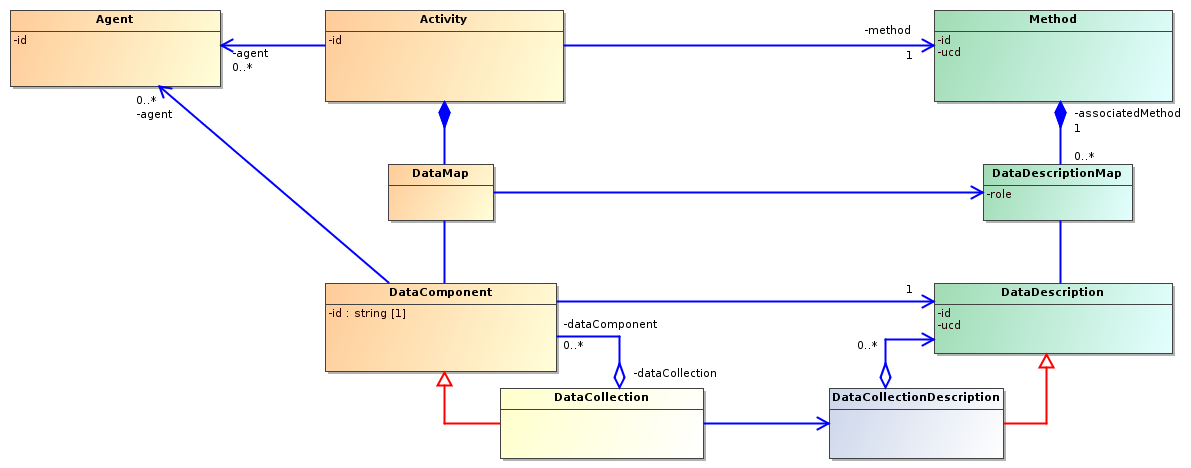
\includegraphics[width=0.8\textwidth]{ProvDM-classdiagram-prototypes.png}
\caption{The class diagram for a provenance data model including prototypes/descriptions for each activity and entity. It will certainly change again, so use it with care. In this version, we stripped it now from nearly all derived classes, so we can concentrate on the core elements. The green and blue boxes belong to ``prototype'' classes.}
\label{fig:classes-prototypes}
\end{figure}


\subsubsection{Activity and method}
As mentioned before, activity corresponds to experiment, and method to protocol from \cite{std:SimDM}.
Some examples for astronomical activities were already given in Section \ref{sec:w3c_overview}, they are processes like observations, post-processing, flat-fielding, correcting bias, astrometric calibration, etc. The method underlying an activity is specified by the corresponding \emph{ActivityDescription} class (previously named \emph{Method}. This could be, for instance, the name of the code used to perform an activity or a more general description of the underlying algorithm. An activity is a concrete case (instance) of using such a method, with a startTime and endTime, and it has to refer to a corresponding method for further information. 

There MUST be exactly one ActivityDescription per Activity. If steps from a pipeline shall be 
grouped together, one needs to create a proper ActivityDescription for describing all 
the steps at once. This method can then be refered to by the pipeline-activity. For grouped activities, also see the next section.

\subsubsection{ActivityCollection}
For facilitating grouping of activities while still making it obvious that this group contains activities, we introduce an \emph{ActivityCollection}, and on its description side also an \emph{ActivityCollectionDescription}. This can be used for describing workflows, instead of using \emph{Plan} as suggested by the W3C model.

\TODO{More details here, why it is useful, what the description-side contains, what not ...}

\subsubsection{DataEntity and DataEntityDescription}
We define a general \emph{DataEntity} class, 
which can represent either an individual data item or a collection of data. The W3C equivalent to this class is called \emph{Entity} only, but we use here \emph{DataEntity} instead, since we do not aim to model cars and abstract ideas here, but more concretely astronomical data of any kind.

\TODO{Decide, if we want to stick to \emph{Entity} instead of \emph{DataEntity} for keeping 
compliance with W3C.}

Following the scheme that each \emph{activity} is described
by its more general \emph{method}, we associate each input or
output data set with a corresponding description of the dataproduct type. 
This just describes the data as it is, its format and content, and could be derived
from other IVOA data models like ObsCore for observations or SSA for spectra.
The DataEntityDescription does NOT contain any information about the usage of the data, 
it tells nothing about them being used as input or output.

\subsubsection{Input/output data, roles for data}
The information on whether data is used as input or was produced as output of 
some activity is given by the \emph{relation-types} between activities and entities.

Each method usually makes assumptions on the structure of input data (FITS file, data
table, binary file of a certain structure ...) and produces a certain form of
output data, which should be described in the general \emph{DataEntityDescription}
class, so that it can be reused for multiple instances of this class.

There has been some dispute (before and at the InterOp in Madrid, May 2014) 
about the different roles of input and output data. Since the results of one 
activity can be input data for
another activity, the structure of input and output data is necessarily the same.
The (annotated) link from an \texttt{Activity} to the corresponding \texttt{DataEntity}
object could tell then if the piece of data is used as input or output. In fact, 
it would be enough to provide this information just for the relations on the description side (right).
%, see Figure~\ref{fig:activities} in section \ref{sec:links_between_data}.

Additionally, input data can take different roles in an activity (auxiliary data like a parameter file, two images, with one that needs to be subtracted from the other) and it must be made explicit which data component needs to fulfull which role in an activity. 
In W3C, this is partially solved by adding a derivation relation between the Entities (data). Here, we have a mapping-class between Activity and DataEntities as well as between ActivityDescription and DataDescription. The mapping-class at the description side, i.e. between the ActivityDescription and its DataEntityDescriptions, contains additionally a role for each relation, e.g. parameter, dark frame, raw image, etc.  If a data set is used as input to an activity or if it results from it, will become clear with these roles.

\Note{For a given ActivityDescription, one could consider pre-defining the necessary/allowed roles already (maybe use an additional class for these), for avoiding that everyone defines his/her own set 
of names for this, so that interoperability can be enhanced.}

Without the mapping tables, the relation between activity/activityDescription and data/dataDescription would be an aggregation relation, or in other words: an association with the aggregationKind ``shared''. That would be required to ensure that all DataEntities linked to an Activity (either as input or output) will survive if the Activity is destroyed, since they are almost always shared with other Activities. 

By using the mapping tables we make the role of a DataEntity in an Activity more explicit and thus can replace the aggregation by a composition relation to the Activity/ActivityDescription and simple associations to the individual data components and their descriptions. 


\subsubsection{Data collections}

There are two major classes of data entities: 

\begin{itemize} 
\item data collections \\e.g. RAVE-DR4 with its databases and database tables, SDSS DR9 with 
all its tables and files, all files from one observing slot\\

\item individual data components\\
e.g. a file, table in a database, parameter value, an image, a fits-file containing a table and image

\end{itemize}


Data can only be grouped to a data collection, if they have the same origin, i.e. if they were
produced by the same activity, so that they have the same basic provenance.

We would leave it to the person/tool recording provenance to decide the level of detail.
With collections, it is possible to just record provenance for e.g. RAVE DR4 as a 
whole, without listing everything that belongs to DR4. The level of detail could be specified in the  DataDescription.

The relation between DataEntity and DataEntityCollection is expressed with a \emph{composite pattern}, 
in the same way as in the W3C model. The DataEntity class includes already the basic properties and functionality for both, data sets like files or 
parameter values or a complete collection. Such common properties are e.g. the link 
to the activity which created the data/dataCollection, a creation date/time and a link to a
storage-object (which is not further specified in this data model).

A DataEntityCollection additionally has links (\emph{hadMember}-relation in W3C) to its 
child-DataEntities, which could again be DataEntityCollections themselves.
This way, one could represent complete data trees, if necessary.

\TODO{W3C does NOT include links from a member of a collection to the collection, but this could be useful to have (for faster look-ups). Include such a link in our model or not?}


\subsubsection{Agent}
In SimDM, someone performing a certain experiment is called \emph{Contact}, 
the W3C provenance data model suggests the term \emph{Agent}, so we adopted it here.
We want to describe someone who is responsible for an activity, e.g. who pressed a button, 
ran a script or performed the observation. The agent could be a single person 
(specified by name), a group of persons (e.g. MUSE WISE Team), project/organization (RAVE) or an institute. 
For each of them a \emph{name} should be specified.

It is desired to have an agent given for each activity, but it
is not enforced (hence 0..*).  It would also increase the value of the given
information if the (current) affiliation of the agent and a project leader/group
leader were specified in order to maximize the chance of finding someone later
on. The agent should not only be used for getting contact information, but also 
to fulfill our ``Attribution'' requirement (Section~\ref{sec:requirements}, 
so that proper credits are given to the right 
people/projects. To this end, we also add a 
relation between a DataEntity and Agent, similar to W3C's 
wasAttributedTo-relation.

Please note, that persons responsible for an activity (e.g. someone calibrating data) are not necessarily also the one's that will be attributed to the resulting data set (this could 
be attributed to the general project for which the person executing the activity is working).

Some examples for possible agent roles are given in Table~\ref{tab:agentroles}
in Section~\ref{sec:w3c-agent}. For comparison, SimDM contains following roles for 
an agent/contact: owner, creator, publisher, contributer.

The roles would be added to the relation between activity/entity and agent, 
i.e. we have here again a mapping class, which allows to reuse the same agent 
with different roles for different activities and entities.


\subsubsection{Storage}
The modelling of storage is not included in this model. 
It would be useful to be able to make a reference from the DataEntity to a storage
object that contains the link to where the data is stored. But we don't fix the 
details here.


\subsubsection{Links, ids}\label{sec:links_between_data}
It would be convenient, if each data object or even each file 
gets a unique id that can be referenced. The W3C provenance model requires ids
for entities, activities and agents, and they have to be qualified strings, 
i.e. containing a namespace. For example, an activity in the RAVE-pipeline could 
have the id \texttt{'rave:radialvelocity\_pipeline'}. Using a namespace for each 
project for these ids will help to make them unique. 

If several copies of a dataset exist, and one of them is corrupted, it would even be useful to know
exactly which copy was used by a given activity. This can be modeled already 
with the existing tools (using a copy-activity), but we doubt that many people
would actually need this level of detail.

\TODO{What about DOI's for datasets? They should be unique. Maybe add another
attribute DOI instead of storageLocation.}


\subsubsection{Calibration data}
The calibration data set consists of images that can be used to calibrate the
raw data. It is not necessary to mention them explicitly in the model, 
they are just another dataSet that is used by activities with a 
calibration-method.


\subsubsection{Ambient conditions}
Ambient conditions are environmental properties, which are special in a way: 
they represent the part of an activity, usually an observation, which cannot be 
(fully) controlled by an
observer, in contrast to other data that can be fully reproduced.
Nevertheless we decided that they can be fully described by our 
dataEntity class already and don't need a separate class in our data model. 

Our model can then also take into account that a certain observation
method requires special ambient conditions, already defined via the 
ActivityDescription (e.g. radio observations rely on different ambient 
conditions than observations
of gamma rays), just following our data - data description scheme.


Ambient conditions are recorded for a certain time (startTime, endTime) and are
usually only valid for a certain time interval. This time interval should be recorded
with a \emph{validity}-attribute for such dataEntities.


\Note{We wondered if ambient conditions could also play a role for some
processing steps or any other activity besides observations? Is there any
additional step performed in which room temperature etc. may play a role and thus
should be recorded? The only example that came to our minds was the storage of
photographic plates, where the humidity and temperature variations can affect the
quality of the photographic plates. But this may be too far from the core use
cases.}



\subsubsection{Instrument characteristics}
In contrast to ambient conditions, instrument characteristics do (usually) not
change from one observation to the other, so they are static, strictly related to
the instrument. 
All the characteristics could be described either as key-value pairs directly with the 
observation (as attributes) or just as datasets, using the DataEntity class. 
One would then 
link the instrument characteristics as a type of input (or output?) data set to a certain 
observation activity. Thus we don't need a separate Instrument or Device class.

\Note{One should also keep in mind that some instrument related parameters can change within time,
e.g. the CCD temperature. The instruments can also change within time because of aging.}


\subsubsection{Quality}
For expressing the quality of data, we could simply define additional 
attributes for each \emph{Activity}
or \emph{DataEntity} object, i.e. zero, one, or more properties in the form of
key-value pairs. We could use a \emph{Quality} namespace to mark a keyword
as quality-related:
\begin{itemize}
    \item quality.comment: [some text]
    \item quality.seeing: [some value]
\end{itemize}
The values could range from a float number to free text.



\subsection{Discussion}
This model was established with having a database implementation in mind. However, the W3C model may offer simpler possibilities to store provenance with the dataEntities themselves, e.g. as an additional extension in fits-headers.

A model using prototypes has the advantage of normalisation: the common processes could be described once and for all at some place (this \emph{some place} is actually the crucial point here!) and then be reused when describing the actual provenance of certain dataEntities and activities.
In an ideal world, ``some place'' could collect all the descriptions from all 
the possible datasets and methods in astronomy, but building such a look-up place is a quite challenging task -- it will probably never be complete. There's also the issue of persistent identifiers/broken links to consider.
Normalisation is useful for closed systems, e.g. for describing the provenance for data produced by a certain pipeline (e.g. MuseWise system) or with workflow tools or when a task needs to be repeated many times. However, the VO is quite the contrary of a closed system and we need to keep an eye on what is actually achievable.

When writing down a simple serialisation of e.g. the provenance for a stacked image with the protoype-model, it soon becomes quite cumbersome to define everything twice: first the descriptions, then the instances. This basically doubles the number of entries to describe provenance (unless there is already some place with all the descriptions to which we can refer).

Expressing provenance for a stacked image with this smaller set of classes may be simpler, but on the other hand constructing a database schema becomes much harder. 
We could leave it to the implementors to choose what is more useful for them, and when extracting provenance, serialising it, then the descriptions are combined with the activity/dataEntity for 
the serialisation, thus probably producing some repetition, but avoiding too many 
links between different items.

\Note{Descriptions could be present in W3C-conform serialisations, if we 
put them into entities.}

\TODO{Check, if PROV-Templates from the W3C (inofficial note) could be used for ActivityDescriptions.}

\section{Applications/Interactions with other Data models}
In this section we discuss how the provenance data model interacts with
other VO data models and how provenance information can be stored.

\section{Accessing provenance information}
\TODO{Add details from the discussion in Paris, 14th April 2016. Francois and 
Mireille had some suggestions for possible ProvDAL and ProvTAP specifications.
\begin{itemize}
\item ProvDAL: retrieve provenance information based on given id of a dataEntity of activity
\item ProvTAP: allows detailed queries for provenance information, discovery of datasets based on 
e.g. code version.
\item Do we need combined query possibilities, i.e. ask for ObsCore-fields and Provenance fields
in one query? Or rather use a 2-step-process, decoupling them from each other?
\end{itemize}
}

\TODO{Also look at PROV-AQ from the W3C.}

\section{Examples}\label{sec:examples}

\subsection{One processing step in PROV-N notation}
\TODO{Put the very simple example here}
See \url{https://volute.g-vo.org/svn/trunk/projects/dm/provenance/description/prov-example-incl-prototypes.txt}
and \url{https://volute.g-vo.org/svn/trunk/projects/dm/provenance/description/prov-example-w3c.txt}


\subsection{Provenance of RAVE database tables (DR4)}
This example shows how the workflow of RAVE data, from images to the final database tables, can be expressed using Provenance. 
The workflow is not included completely, only some major steps are taken into account. It shows that the provenance concepts explained in this draft can be applied directly to data obtained from astronomical observations.

\TODO{Include here figure from InterOp talk. See also https://provenance.ecs.soton.ac.uk/store/documents/84064/}

\subsection{POLLUX database}

\subsection{CTA provenance}


\section{Implementations}
\TODO{Maybe combine with examples?}


\appendix
\section{Changes from Previous Versions}
No official previous versions yet.
% No previous versions yet.  
% these would be subsections "Changes from v. WD-..."
% Use itemize environments.


\bibliography{ivoatex/ivoabib,prov-refs}


\end{document}
